

\section{Введение}
Во время различных научных экспериментов часто возникает задача определить некоторую физическую величину при помощи измерительных приборов. При измерении  невозможно получить ее абсолютно точное значение, так как не существует идеальных измерительных инструментов и методов.

По этой причине, после произведённого измерения физической величины, нужно указать погрешность измерения.

На значение конкретного измерения влияют систематические и случайные погрешности. Их источниками могут являться сами измерительные приборы. Кроме того, погрешность может возникать из-за несовершенства методики измерения и промахов самого экспериментатора. 
Для качественной оценки погрешности необходимо многократно измерять нужную величину.


\subsection{Задачи работы}

Таким образом, задачами данной работы являются:
\begin{enumerate}
    \item Освоить методику использования измерительного прибора для
многократного прямого измерения физической величины.
    \item Выполнить простейшую статистическую обработку серии
результатов наблюдений при прямых измерениях.

\end{enumerate}




\section{Основная часть}

\subsection{Теоретическая часть}
Для оценки погрешности измерения физическую величину необходимо измерить несколько раз. Таким образом, будет получена соответствующая выборка:


\begin{equation}
    x_1,x_2,x_3, ..., x_n
\end{equation}
Значения из выборки отличаются от истинного значения измеряемой физической величины. Это вызвано влиянием погрешностей на каждое единичное измерение.\\
Необходимо определить, что целесообразнее всего считать результатом измерения. В качестве оптимального значения измеряемой величины (то есть результата измерения) принимается среднее арифметическое.
\begin{equation}
    \overline{x}=\frac{x_1+x_2+...+x_n}{n}=\frac{1}{n}\sum_{i=1}^{n} x_i
\end{equation}
Приняв, что измеряемая величина равна среднему значению, можно производить дальнейший анализ полученных данных. Стоит убедиться в отсутствии дрейфа - изменением значений с течением времени.
Дальнейший анализ полученной выборки состоит в рассмотрении распределения результатов наблюдения с помощью гистограммы, графика зависимости или наблюдении результатов на числовой оси.\\
С помощью графика зависимости можно определить дисперсию распределения (среднюю квадратическую погрешность отдельного наблюдения). Кроме того, дисперсию можно найти по приближенной формуле (6):
\begin{equation}
    \sigma=\sqrt{\frac{1}{n-1}\sum_{i=1} (x_i-\overline{x})^2}
\end{equation}
Средняя квадратичная погрешность среднего связана с дисперсией следующей формулой:
\begin{equation}
    \sigma_{\overline{x}}=\frac{\sigma}{\sqrt{n}} ,
\end{equation}
где n - число измерений.
Интервал, внутрь которого с заданной вероятностью попадает истинное значение задаётся следующим выражением:
\begin{equation}
    x=\overline{x}\pm\sigma_{\overline{x}} ,
\end{equation}


\subsection{Эксперимент}
Лабораторная работа заключается в измерении  электронным частотомером ЧЗ-32 частоты следования импульсов.\\ От генератора сигналов на частотомер подается последовательность
прямоугольных импульсов, заданных параметров. Частота следования импульсов измеряется с помощью частотомера на двух
шкалах: грубой и точной. В качестве генератора импульсов используется
генератор Г5-15, а в качестве частотомера – Ч3—32.\\
Схема установки приведена на рис.~\ref{fig:Схема установки}. На рис.~\ref{fig:установка} представлена фотография установки, сделанная во время проведения лабораторной работы.

\begin{figure}[H]
\centering
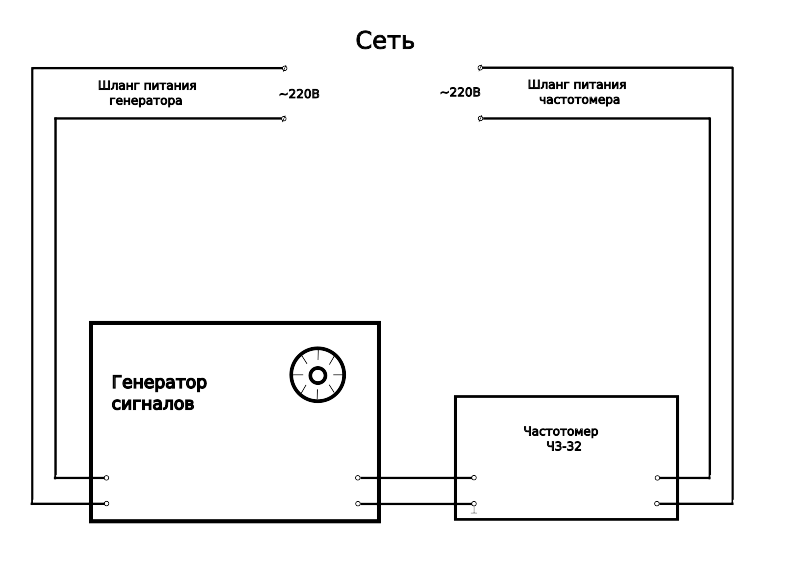
\includegraphics[width=0.8\textwidth]{Схема установки}
\caption{Схема установки}
\label{fig:Схема установки}
\end{figure}



\begin{figure}[H]
\centering
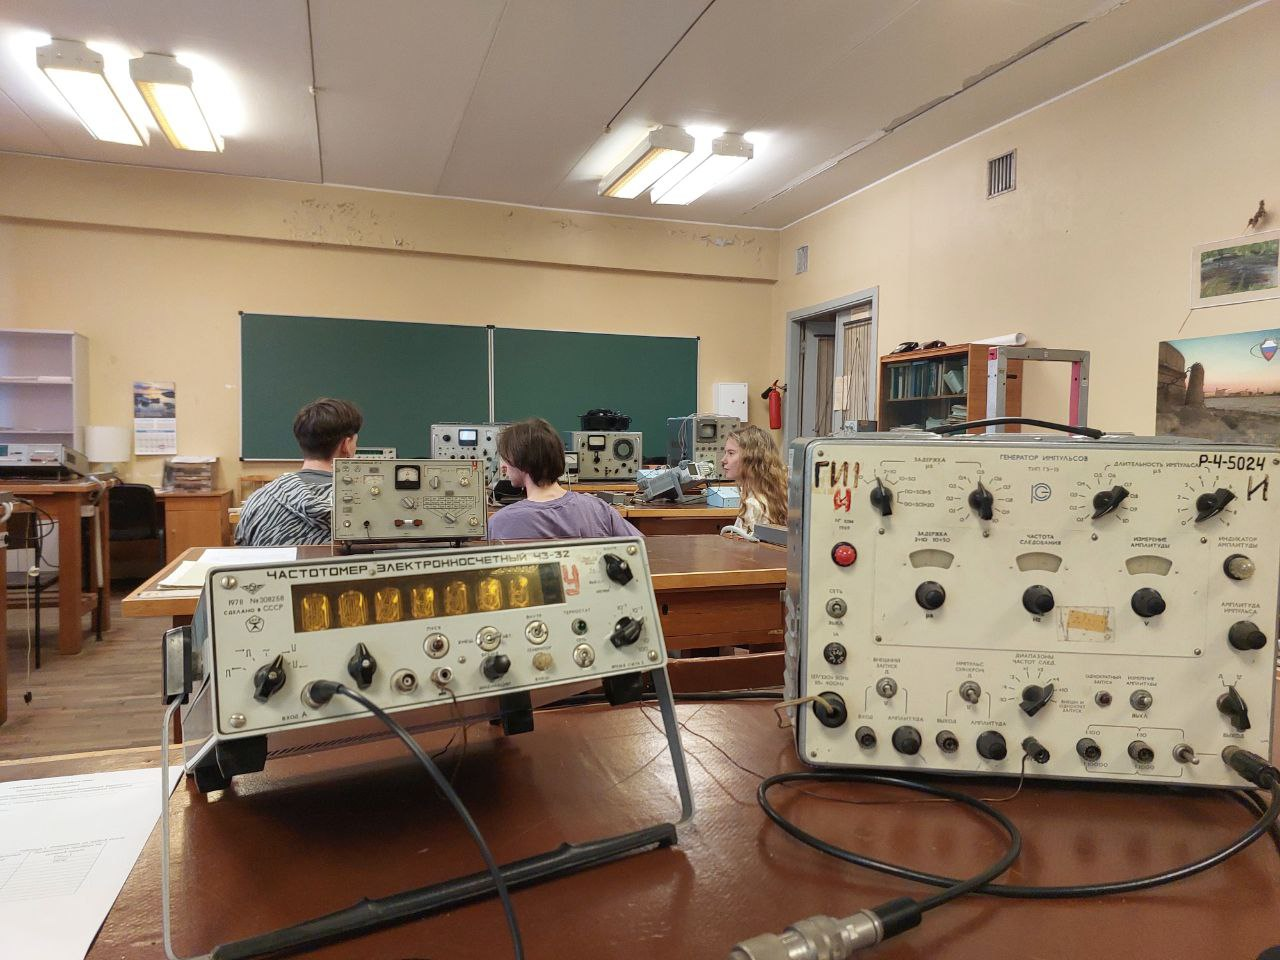
\includegraphics[width=0.8\textwidth]{Установка.jpg}
\caption{Установка}
\label{fig:установка}
\end{figure}

\subsection{Обработка данных и обсуждение результатов}
Вычисление погрешности прибора $\Delta f$ производится по следующим формулам:
\begin{equation}
   \gamma_f=  \frac{\Delta f}{f_x}*100\%
\end{equation}
\begin{equation}
 \gamma_f=\pm(\gamma_0+\frac{1}{(f_x*T)})*100,
 \end{equation}
 где $\gamma_f$ - относительная погрешность прибора, $\gamma_0$=$\pm$$5*10^{-7}$, T=0.1 с на грубой шкале, T=1 с на точной шкале.\\
 На грубой шкале было произведено 10 измерений, результаты представлены в таблице ~\ref{tabl:1}.

\begin{center}
\begin{table}[h!]
\centering
\caption{Измерения на грубой шкале}
\label{tabl:1}
\begin{tabular}{|c|c|c|c|c|}
\hline
\begin{minipage}{7mm}
    № п.п. 
\end{minipage}&
\begin{minipage}{5cm}
    Диапазон показаний использованной шкалы прибора
\end{minipage} &
\begin{minipage}{5cm}
    Результаты отдельных наблюдений ($f_i$)
\end{minipage} &
\begin{minipage}{5cm}
    Погрешность прибора на данной шкале ($\Delta f_{\text{приб}}$)
\end{minipage}\\
\hline
{}&кГц&кГц&кГц\\
\hline
1 &  0-10^5  &  4.56  &  0.0102 \\
2 &  0-10^5  &  4.54  &  0.0102 \\
3 &  0-10^5  &  4.54  &  0.0102 \\
4 &  0-10^5  &  4.56  &  0.0102 \\
5 & 0-10^5  &  4.56  &  0.0102 \\
6 & 0-10^5  &  4.56  &  0.0102 \\
7 & 0-10^5  &  4.58  &  0.0102 \\
8 & 0-10^5  &  4.56  &  0.0102 \\
9 & 0-10^5  &  4.58  &  0.0102 \\
10& 0-10^5  &  4.56  &  0.0102 \\
\hline
\end{tabular}
\end{table}
\end{center}
Так же было получено $\overline{f}$=4.56 кГц.\\

На точной шкале погрешность прибора $\Delta f_{\text{приб}}$ составила 0.001000 кГц.
Результаты 50 измерений, произведенных на точной шкале представлены в таблице ~\ref{tabl:2}.
\begin{center}
\begin{table}[H]
\centering
\caption{Измерения на точной шкале}
\label{tabl:2}
\begin{tabular}{|c|c|c|c|c|}
\hline
\begin{minipage}{7mm}
    № п.п. 
\end{minipage}&
\begin{minipage}{5cm}
    Результаты отдельных наблюдений ($f_i$)
\end{minipage} &
\begin{minipage}{5cm}
    Случайные отклонения от среднего d_i=$f_i-\overline{f}$
\end{minipage} &
\begin{minipage}{5cm}
    Погрешность прибора на данной шкале d_i^2=($f_i-$$\overline{f}$)^2
\end{minipage}\\
\hline
{}&кГц&кГц&кГц^2\\
\hline
1  &    4.566  &  0.022 & 0.000484 \\
2  &    4.564  &  0.020 & 0.000400 \\
3  &    4.564  &  0.020 & 0.000400 \\
4  &    4.563  &  0.019 & 0.000361 \\
5  &    4.562  &  0.018 & 0.000324 \\
6  &    4.564  &  0.020 & 0.000400 \\
7  &    4.550  &  0.006 & 0.000036 \\
8  &    4.542  &  -0.002 & 0.000004 \\
9  &    4.540  &  -0.004 & 0.000016 \\
10 &  4.538  &  -0.006 & 0.000036 \\
11 &  4.542  &  -0.002 & 0.000004 \\
12 &  4.542  &  -0.002 & 0.000004 \\
13 &  4.542  &  -0.002 & 0.000004 \\
14 &  4.540  &  -0.004 & 0.000016 \\
15 &  4.542  &  -0.002 & 0.000004 \\
16 &  4.542  &  -0.002 & 0.000004 \\
17 &  4.542  &  -0.002 & 0.000004 \\
18 &  4.542  &  -0.002 & 0.000004 \\
19 &  4.542  &  -0.002 & 0.000004 \\
20 &  4.542  &  -0.002 & 0.000004 \\
21 &  4.544  &  0.000 & 0.000000 \\
22 &  4.544  &  0.000 & 0.000000 \\
23 &  4.544  &  0.000 & 0.000000 \\
24 &  4.544  &  0.000 & 0.000000 \\
25 &  4.544  &  0.000 & 0.000000 \\
26 &  4.542  &  -0.002 & 0.000004 \\
27 &  4.542  &  -0.002 & 0.000004 \\
28 &  4.540  &  -0.004 & 0.000016 \\
29 &  4.540  &  -0.004 & 0.000016 \\
30 &  4.542  &  -0.002 & 0.000004 \\
31 &  4.540  &  -0.004 & 0.000016 \\
32 &  4.542  &  -0.002 & 0.000004 \\
33 &  4.540  &  -0.004 & 0.000016 \\
34 &  4.540  &  -0.004 & 0.000016 \\
35 &  4.540  &  -0.004 & 0.000016 \\
36 &  4.538  &  -0.006 & 0.000035 \\
37 &  4.540  &  -0.004 & 0.000016 \\
38 &  4.540  &  -0.004 & 0.000016 \\
\end{tabular}
\end{table}
\end{center}
\begin{center}
\begin{table}[H]
\centering

\label{tabl:11}
\begin{tabular}{|c|c|c|c|c|}
\hline
\begin{minipage}{7mm}
    № п.п. 
\end{minipage}&
\begin{minipage}{5cm}
    Результаты отдельных наблюдений ($f_i$)
\end{minipage} &
\begin{minipage}{5cm}
    Случайные отклонения от среднего d_i=$f_i-\overline{f}$
\end{minipage} &
\begin{minipage}{5cm}
    Погрешность прибора на данной шкале d_i^2=($f_i-$$\overline{f}$)^2
\end{minipage}\\
\hline
{}&кГц&кГц&кГц^2\\
\hline
39 &  4.540  &  -0.004 & 0.000016 \\
40 &  4.540  &  -0.004 & 0.000016 \\
41 &  4.540  &  -0.004 & 0.000016 \\
42 &  4.538  &  -0.006 & 0.000036 \\
43 &  4.540  &  -0.004 & 0.000016 \\
44 &  4.538  &  -0.006 & 0.000036 \\
45 &  4.540  &  -0.004 & 0.000016 \\
46 &  4.538  &  -0.006 & 0.000036 \\
47 &  4.538  &  -0.006 & 0.000036 \\
48 &  4.538  &  -0.006 & 0.000036 \\
49 &  4.542  &  -0.002 & 0.000004 \\
50 &  4.541  &  -0.003 & 0.000009 \\
\hline
   &  $\overline{f}$=4.544 & d_i=0.004 & $d_i^2=0.0002907$\\
\hline
\end{tabular}
\end{table}
\end{center}

\subsubsection{Графики}

На рис.~\ref{fig:graph1} приведён график зависимости результатов наблюдений от времени.
\begin{figure}[H]
\centering
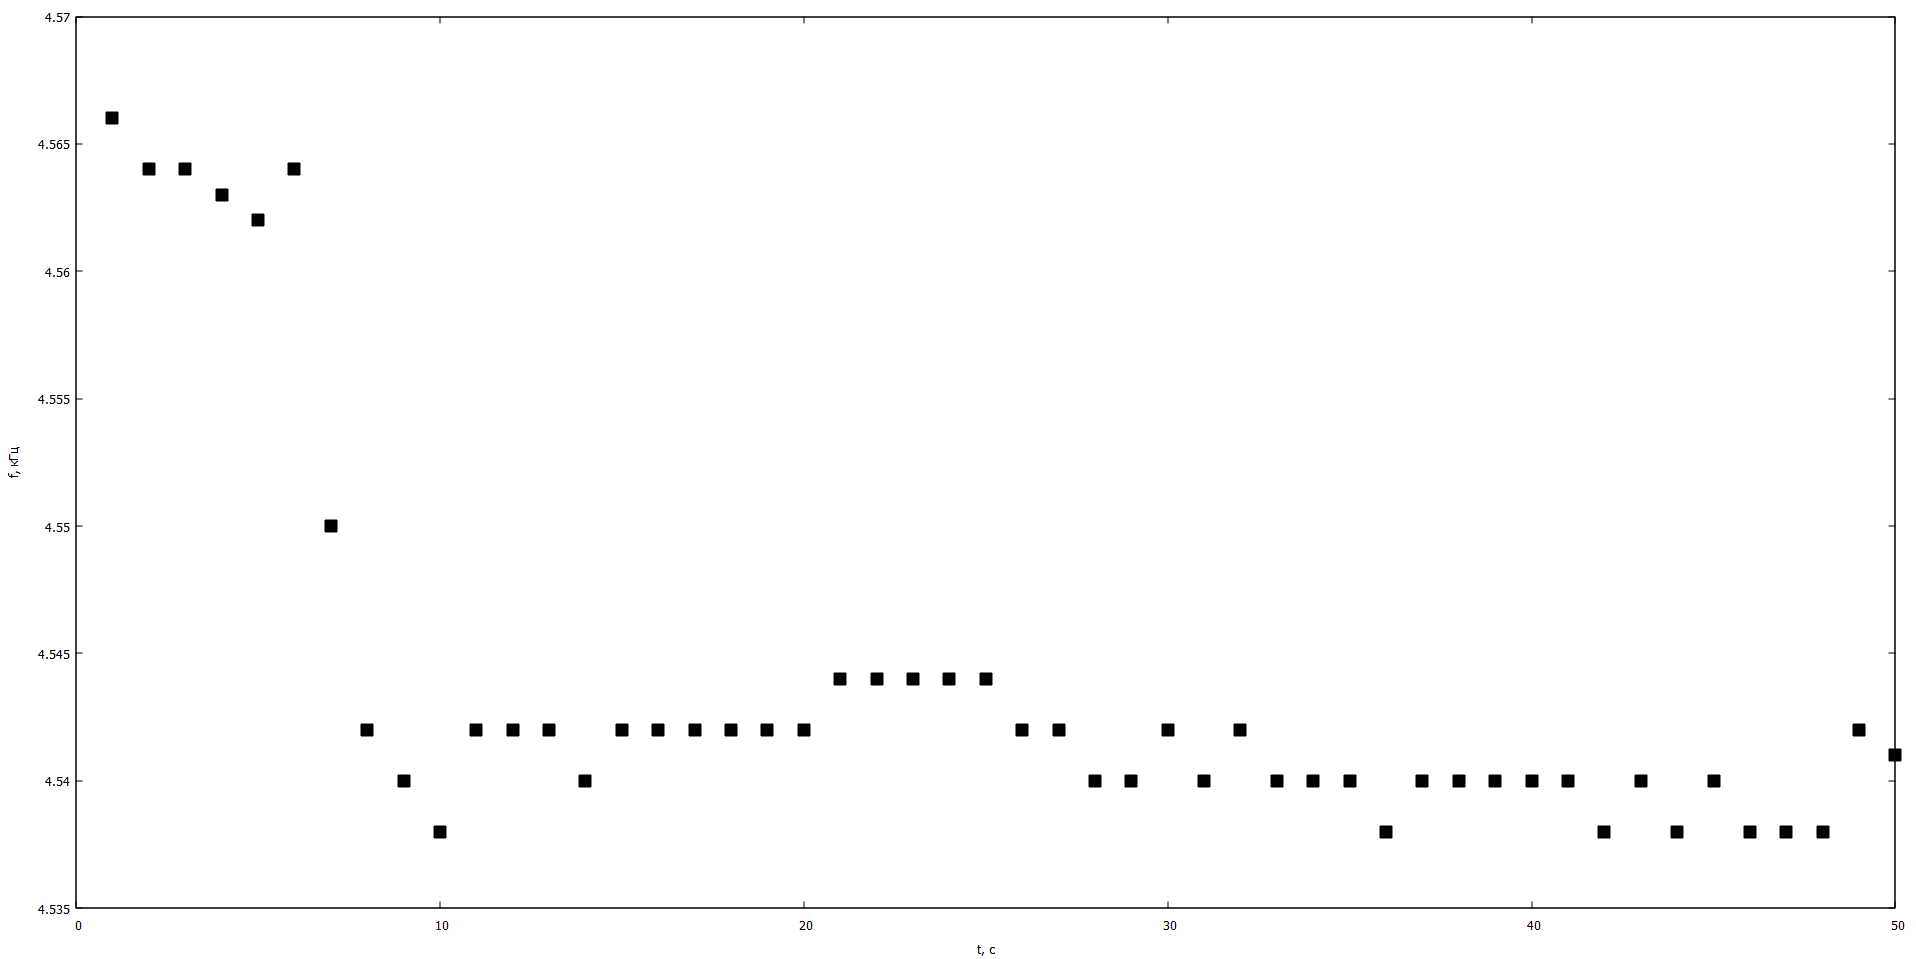
\includegraphics[width=1.0\textwidth]{graph1}
\caption{Зависимость результатов наблюдений от времени}
\label{fig:graph1}
\end{figure}

На рис.~\ref{fig:graph2} представлено распределение результатов наблюдений на числовой оси.
\begin{figure}[H]
\centering
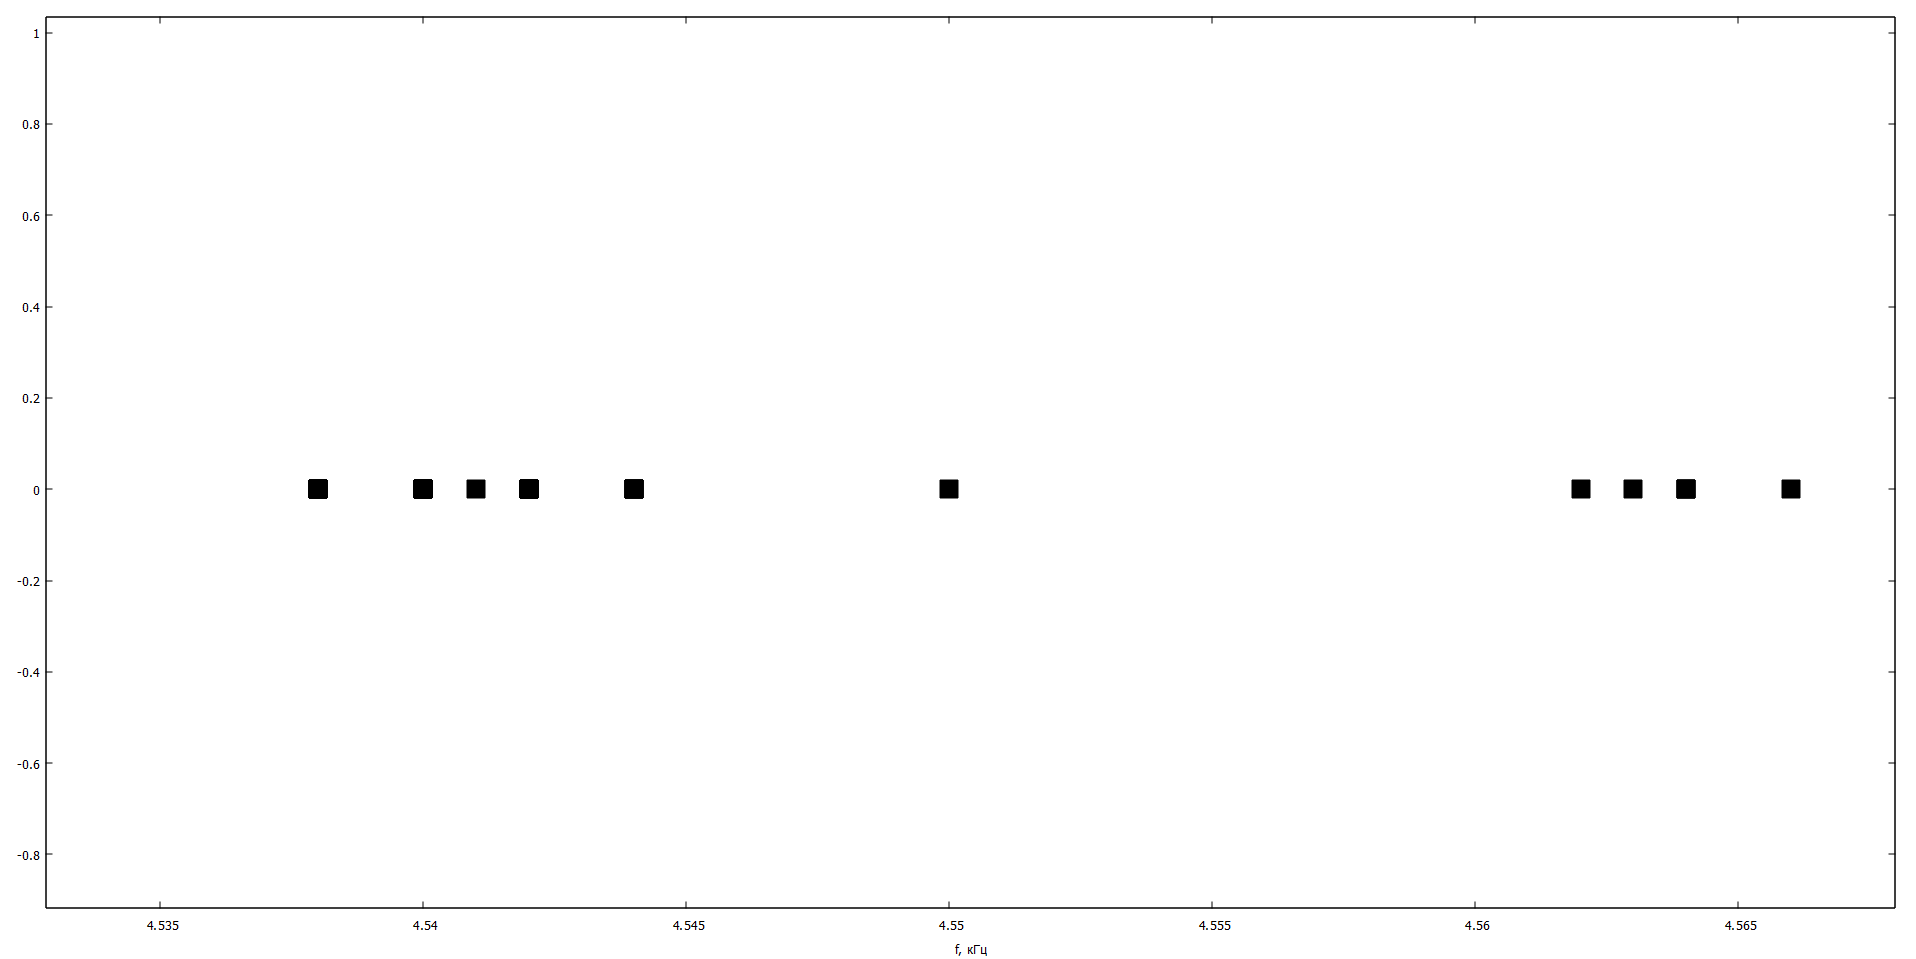
\includegraphics[width=1.0\textwidth]{graph2}
\caption{Распределение результатов наблюдений на числовой оси}
\label{fig:graph2}
\end{figure}
\begin{center}
\begin{table}[H]
\centering
\label{tabl:3}
\caption{Таблица распределения результатов}
\begin{tabular}{|c|c|c|c|c|}
\hline
\begin{minipage}{2cm}
    Номер интервала
\end{minipage}&
\begin{minipage}{3cm}
    Границы интервалов
\end{minipage} &
\begin{minipage}{5cm}
    Число случаев($\Delta n$), когда результат наблюдения попадает в данный интервал
\end{minipage} &
\begin{minipage}{5cm}
    Доля (часть) полного числа результатов, попадающих в этот интервал $\delta n=\frac{\Delta n}{n}$
\end{minipage}\\
\hline
1 &  [4.538,4.542)  &  23 & 0.46 \\
2 &  [4.542,4.546)  &  20 & 0.4 \\
3 &  [4.546,4.550)  &  1 & 0.02 \\
4 &  [4.550,4.554)  &  0 & 0 \\
5 &  [4.554,4.568) &  0 & 0 \\
6 &  [4.568,4.562)  &  2 & 0.04 \\
7 &  [4.562,4.566)  &  4 & 0.08 \\

\hline
\end{tabular}
\end{table}
\end{center}\\

\begin{figure}[H]
\centering
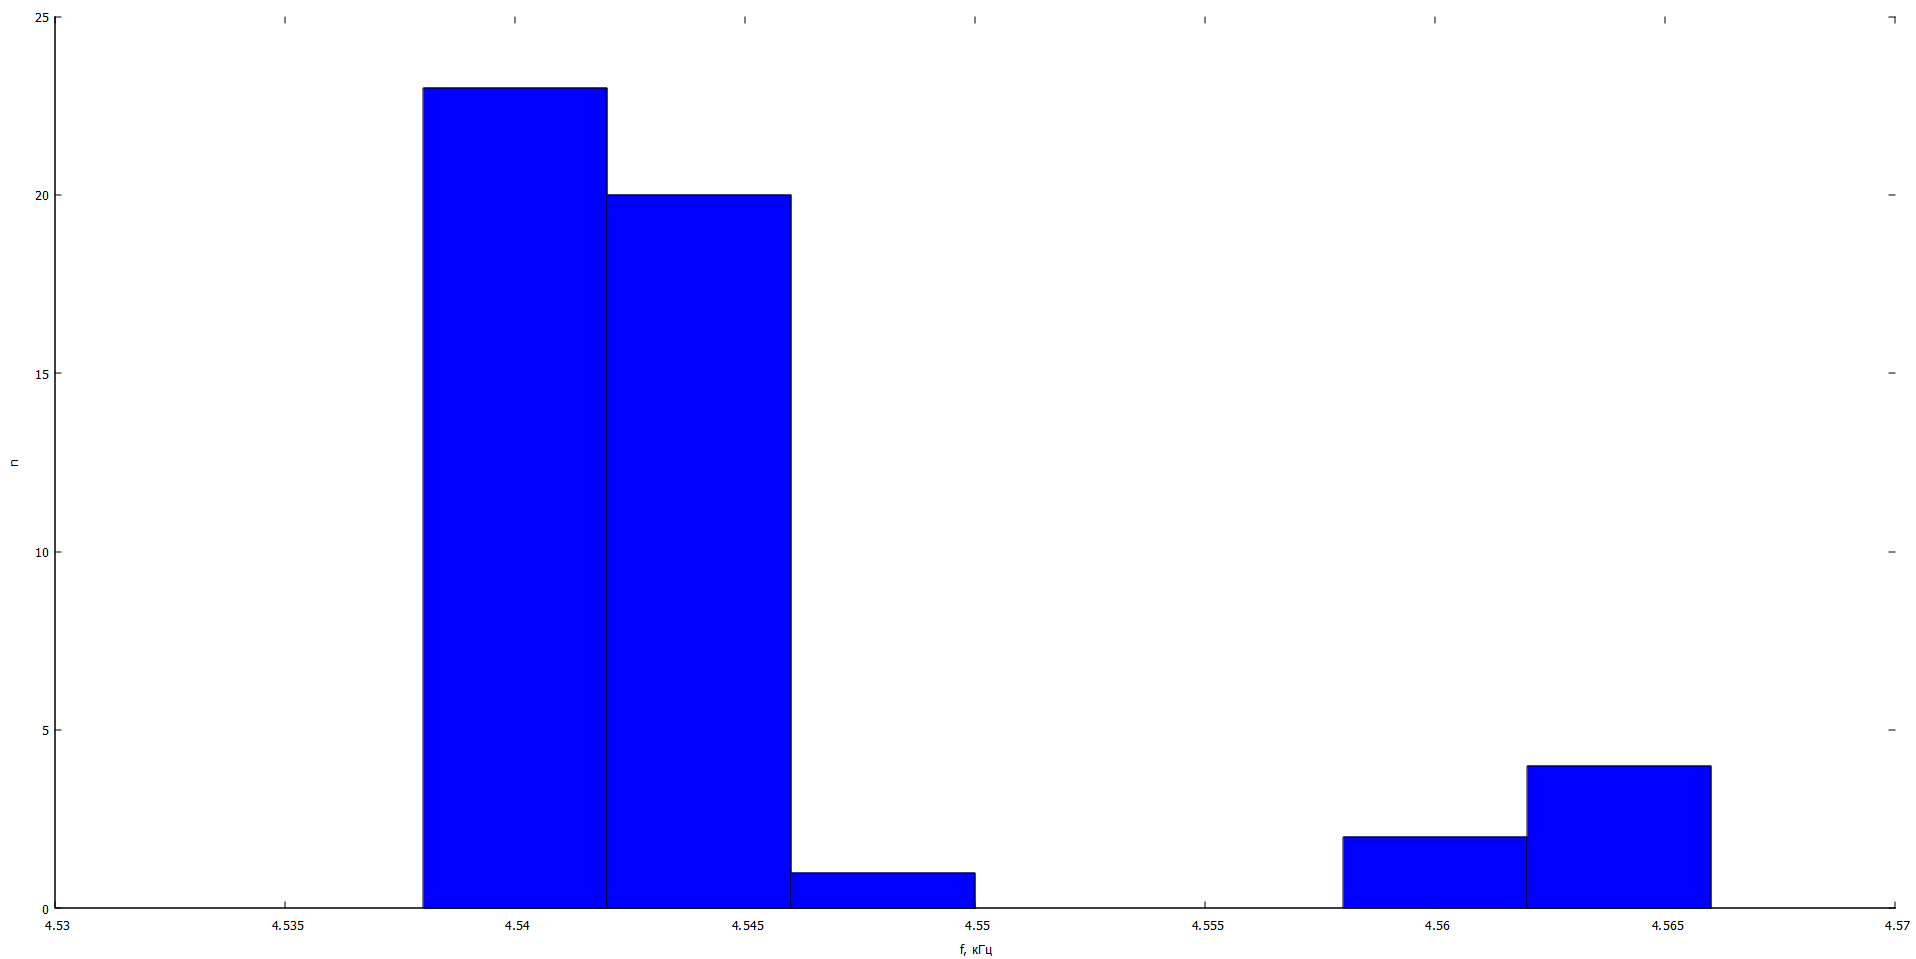
\includegraphics[width=1.0\textwidth]{gist}
\caption{Распределение результатов наблюдений: гистрограмма}
\label{fig:gist}
\end{figure}
\begin{figure}[H]
\centering
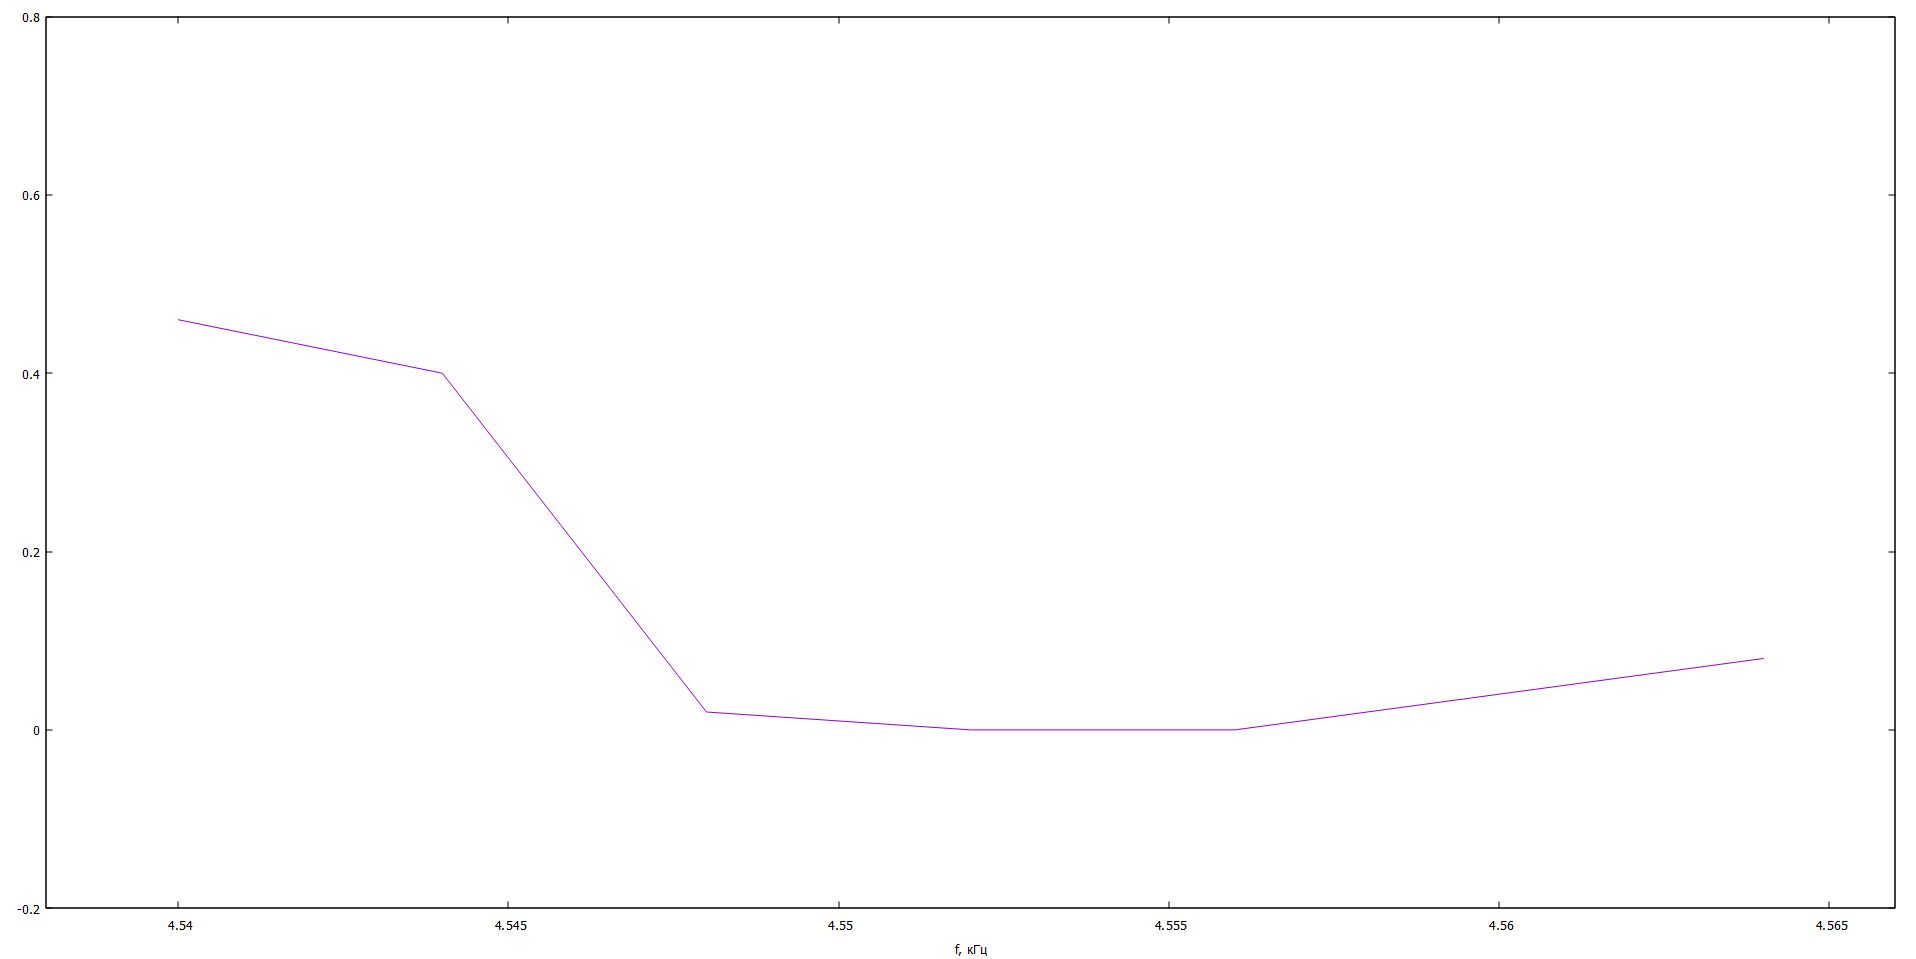
\includegraphics[width=1.0\textwidth]{graph3}
\caption{Распределение результатов наблюдений: график}
\label{fig:graph3}
\end{figure}\\
Высчитанные величины:\\
Дисперсия: $\sigma=0.007780$\\
Средняя квадратичная погрешность среднего: $\sigma_f$=0.001100\\
$f=4.544\pm0.001100$\\
Так как случайная и системная погрешность одного порядка, применяем формулу:
Суммарная погрешность: $\sigma_{сумм}=\sqrt{(\frac{\Delta f_{прибора}}{3})^2+\sigma_f^2}$\\
$\sigma_{сумм}=0,001065$
\section{Выводы}
В процессе этой лабораторной работы я ознакомился с методиками использования прибора (частотомера ЧЗ-32) для многократного измерения частоты. Кроме этого, я научился выполнять анализ, полученных данных, путём построения таблиц распределения, графиков, гистограмм; вычислять дисперсию, среднюю квадратичную погрешность среднего.
\section{Ссылки}
Исходный код - https://github.com/st117207/Workshop1


